\section{DTM Extraction}

To Train a model to derive a DTM from point cloud data and then use this DTM to estimate natural surface water flow patterns and design drainage plans for the region.

Key considerations for the solution plan include:
\begin{itemize}
	\item Tree canopy obscuring the ground in point cloud data, making it difficult to derive an accurate DTM.
	\item Tree canopu will be smoothed using neraby ground points.
	\item buildings and other manmade structures will be reatained in the DTM to ensure accurate surface water flow estimation and drainage planning.
\end{itemize}

Figure \ref{fig:solution_plan} illustrates the training workflow for DTM extraction, while Figure \ref{fig:solution_plan_inference} illustrates the inference workflow for DTM extraction. 


\subsection{DTM extraction (Training)}

SMRF (Simple Morphological Filter) from the PDAL library will be used to classify ground points in the point cloud data. 
sklearn library will be used to impute Z values for unclassified points to simulate the plain Terrain beneath the tree canopy. 
This will help in generating a more accurate DTM that captures the underlying terrain features, which is crucial for surface water flow estimation and drainage planning.
An Encoder-Decoder transformer architecture will be trained for DTM extraction, using the point cloud data as input and the derived DTM as output. on selected spatial windows of the point cloud data (Manually generated AOI where the tree canopy is pesent).
The model will learn to capture the complex relationships between the point cloud data and the underlying terrain features, enabling it to generate accurate DTMs even in areas with dense tree canopy or other obstructions.


\begin{figure}
	\centering
	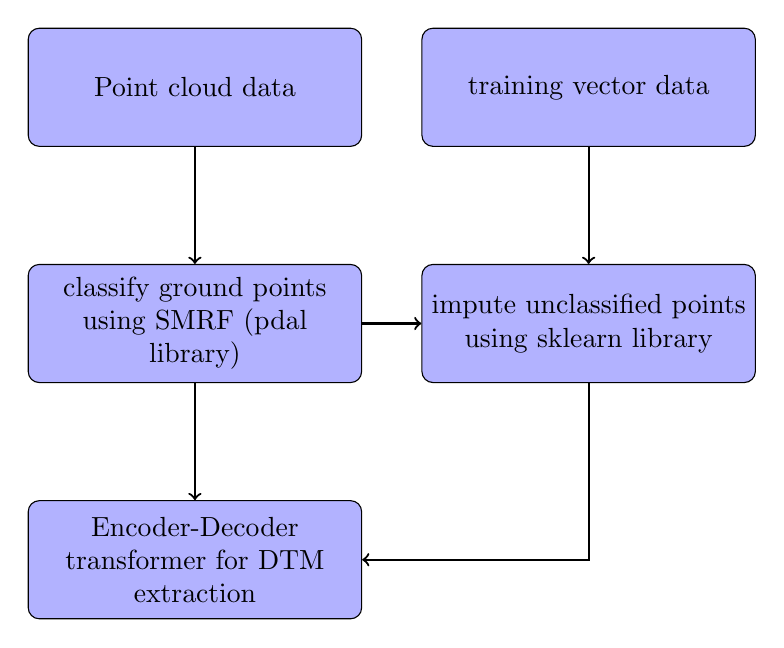
\begin{tikzpicture}
		\tikzstyle{block} =[ draw, text width = 4cm, minimum height=1.5cm, text badly centered, rounded corners, fill=blue!30];
		\node[block] (las) {Point cloud data};    
		\node[block, below of = las, node distance=3cm] (smrf) {classify ground points using SMRF (pdal library)};  
		\node[block, below of = smrf, node distance=3cm]  (transformer) {Encoder-Decoder transformer for DTM extraction};
		\node[block, right of = smrf, node distance=5cm] (impute) {impute unclassified points using sklearn library};
		\node[block,above of = impute, node distance=3cm] (vector) {training vector data};
		
		\draw[->,thick] (las) -- (smrf);
		\draw[->,thick] (vector) -- (impute);
		\draw[->,thick] (smrf) -- (transformer);
		\draw[->,thick] (impute) |- (transformer);
		\draw[->,thick] (smrf) -- (impute);
	\end{tikzpicture}
	\caption{DTM extraction training workflow}
	\label{fig:solution_plan}
\end{figure}



\subsection{DTM extraction (Inference)}

The trained Encoder-Decoder transformer model will be used to derive DTMs from new point cloud data during inference.
The point cloud data will be processed in spatial windows to manage computational resources effectively.
The model will generate DTM outputs for each spatial window, which can then be combined to create a comprehensive DTM for the entire area of interest. 
This DTM will serve as the basis for subsequent surface water flow estimation and drainage planning tasks, enabling informed decision-making for effective water management in the region.

\begin{figure}
	\centering
	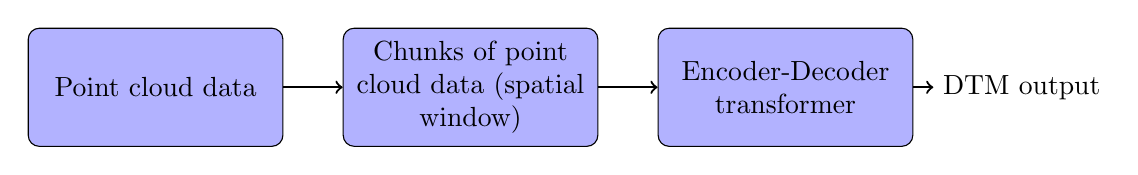
\begin{tikzpicture}
		\tikzstyle{block} =[ draw, text width = 3cm, minimum height=1.5cm, text badly centered, rounded corners, fill=blue!30];
		\node[block] (las) {Point cloud data};    
		\node[block, right of = las, node distance=4cm] (spatialwindow) {Chunks of point cloud data (spatial window)};  
		
		\node[block, right of = spatialwindow, node distance=4cm]  (transformer) {Encoder-Decoder transformer};
		\node[right of = transformer, node distance=3cm] (DTM output){DTM output};
		
		\draw[->,thick] (las) -- (spatialwindow);
		\draw[->,thick] (spatialwindow) -- (transformer);
		\draw[->,thick] (transformer) -- (DTM output);
	\end{tikzpicture}
	\caption{DTM extraction inference workflow}
	\label{fig:solution_plan_inference}
\end{figure}



\subsection{Results and evaluation}

\begin{figure}
	\centering
	\includegraphics{AOI_knn_id2.png}
	\caption{AOI for training data generation using knn imputation}
	\label{fig:AOI_knn}
\end{figure}

\begin{figure}
	\centering
		\begin{subfigure}{\textwidth}
		
\includegraphics[width=0.8\textwidth]{paraview_dsm_id_2.png}
		\caption{Input point cloud data (DSM)}
		\end{subfigure}

		\begin{subfigure}{\textwidth}
		
\includegraphics[width=0.8\textwidth]{paraview_dtm_id_2.png}
		\caption{Derived DTM from the trained model}
		\end{subfigure}

		\begin{subfigure}{\textwidth}
		
\includegraphics[width=0.8\textwidth]{paraview_ismr_id_2.png}
		\caption{Ground points classified by SMRF}			
		\end{subfigure}
	\caption{DTM extraction using knn imputation for training data generation}

	\label{fig:dtm_results}
\end{figure}